% \vspace{-1.5em}
% \begin{wrapfigure}{r}{0.7\textwidth}
%     \centering
%     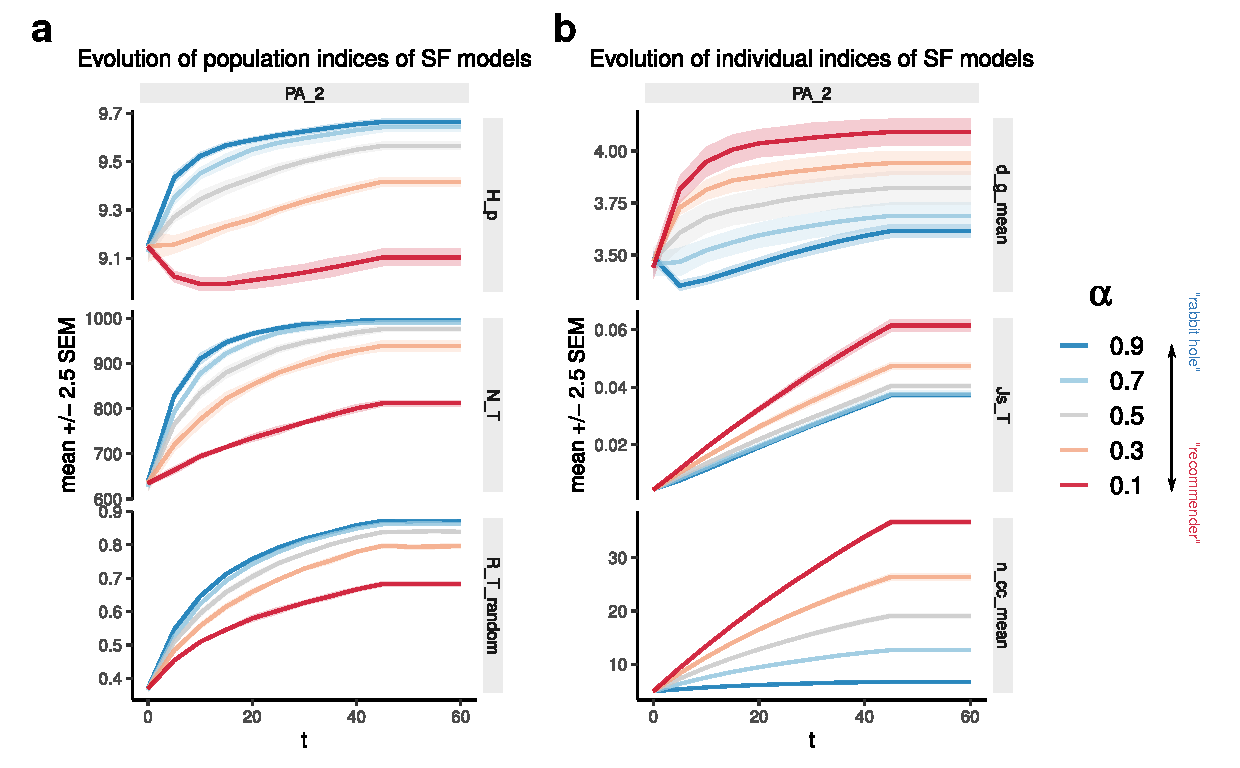
\includegraphics[width=0.7\textwidth,center]{../figures/report/Fig3.pdf}
\begin{figure}
    \centering
    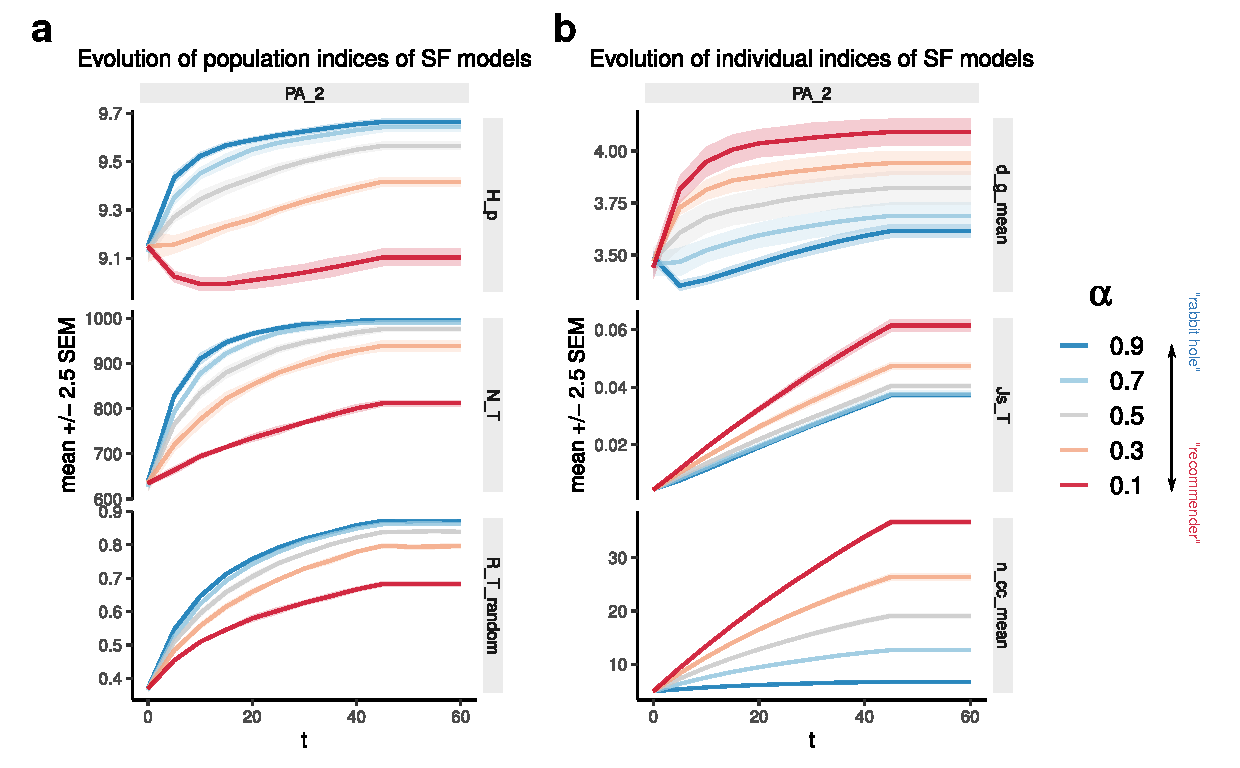
\includegraphics[width=0.7\textwidth,center]{../figures/report/Fig3.pdf}
    \caption{\label{fig:3}
    \textit{Changes of population diversity indices} (\textbf{a}) \textit{and of individual diversity indices} (\textbf{b}) \textit{of the scale-free intralayer models} ($PA_2$) \textit{due to} $\alpha$. $H_p$: topic population entropy; $N_T$: number of distinct topics; $R_T$: robustness due to random removal of agents; $d_g$: mean distance of the subset of topics that agents know; $Js_T$: Jaccard similarity of topic set between agents; $n_{\mathrm{cc}}$: number of connected components of induced subgraphs based on each agent's learnt topics. See method for detailed description.
%     \vspace{-1.5em}
    }
\end{figure}
% \end{wrapfigure}\leavevmode
